\documentclass[11pt,a4paper,spanish]{book}
\usepackage{estilo_unir-1}
\usepackage{apacite}

\usepackage{hyperref}
\numberwithin{equation}{chapter}
%\usepackage{caption}
\numberwithin{figure}{chapter}
%\usepackage{chngcntr}
%\counterwithin{equation}{chapter}
%\counterwithin{figure}{chapter}
%\counterwithin{table}{chapter}
%\renewcommand\theequation{\thechapter.\arabic{equation}}
%\renewcommand\thefigure{\thechapter.\arabic{figure}}
%\renewcommand\thetable{\thechapter.\arabic{table}}
%\renewcommand\theequation{\thechapter.\arabic{equation}}
%\counterwithin{figure}{chapter}
%\counterwithin{table}{chapter}
%\renewcommand\thefigure{\thechapter.\arabic{figure}}
%\renewcommand\thetable{\thechapter.\arabic{table}}
%\renewcommand\thefigure{\thechapter.\arabic{figure}}
%\makeatletter
%\renewcommand\p@figure{\thechapter..\arabic{figure}}
%\makeatother



%---------------------------
%título del trabajo y autor
%---------------------------
\title{Reconocimiento de patrones en sistemas industriales para la detección de fallos
		mediante algoritmos de Aprendizaje Automático}
\titulacion{Máster Universitario en Inteligencia Artificial}
\author{Jorge Elicer Lambraño Arroyo}
\date{11 de Septiembre de 2025}
\director{Gabriel Mauricio Ramírez Villegas}
\nombreciudad{Bogotá (Colombia)}

%---------------------------
%marges
%---------------------------
%\usepackage[margin=1.9cm]{geometry}
%---------------------------
%---------------------------
%---------------------------
%---------------------------
\begin{document}
\renewcommand{\listfigurename}{Índice de Ilustraciones}
\renewcommand{\listtablename}{Índice de Tablas}
\renewcommand{\contentsname}{Índice de Contenidos}
\renewcommand{\figurename}{Figura}
\renewcommand{\tablename}{Tabla} 

\maketitle

\frontmatter
\tableofcontents
\listoffigures
\listoftables

\chapter{Resumen}
% {\bf Nota:} En este apartado se introducirá un breve resumen en español del trabajo 
% realizado (extensión máxima: 150 palabras). Este resumen debe incluir el objetivo o 
% propósito de la investigación, la metodología, los resultados y las conclusiones.
El presente proyecto aborda la temática de  la detección de anomalías en rodamientos 
utilizando el CWRU Bearing Dataset como fuente de información. El objetivo principal 
consiste en comparar el desempeño de diversos modelos de aprendizaje automático con el 
fin de identificar cuál resulta más apropiado para el desarrollo de un detector de 
anomalías robusto, eficiente y aplicable en entornos industriales. Para ello, se 
implementaron diferentes etapas de preprocesamiento,  caracterización de las señales 
temporales y estrategías durante la fase el entrenamiento de los modelos, con el 
propósito de obtener un modelo optimizado con altas métricas de rendimiento que facilite
la tarea de detección de anomalías.Los resultados alcanzaron métricas superiores al 
90\% de exactitud, precisión, sensibilidad, F1-score y área bajo la curva RoC, lo que 
demuestra la viabilidad de aplicar machine learning en la detección temprana de fallas
en rodamientos

{\bf Palabras Clave:} Aprendizaje automático; CWRU Bearing Dataset; Detección de anomalías;
Mantenimiento predictivo; Series de tiempo.

\chapter{Abstract}
% {\bf Nota:} En este apartado se introducirá un breve resumen en español del trabajo
% realizado (extensión máxima: 150 palabras). Este resumen debe incluir el objetivo o 
% propósito de la investigación, la metodología, los resultados y las conclusiones.
The present project addresses the topic of anomaly detection in bearings using the CWRU
Bearing Dataset as the source of information. The main objective is to compare the 
performance of various machine learning models in order to identify which one is the most
suitable for the development of a robust, efficient, and industrially applicable anomaly
detector. To this end, different preprocessing stages, time-series signal characterization,
and training strategies were implemented with the purpose of obtaining an optimized model
with high performance metrics that facilitates the anomaly detection task. The results 
achieved over 90\% in accuracy, precision, recall, F1-score and RoC curve, demonstrating
the feasibility of applying machine learning for early fault detection in bearings.

{\bf Palabras Clave:} Machine Learning; CWRU Bearing Dataset; Anomaly detectino;
Predictive maintenance; Time series.




\mainmatter
\chapter{Introducción}

% El primer capítulo es siempre una introducción. En la introducción se debe resumir 
% de forma esquemática % pero suficientemente clara lo esencial de cada una de las partes 
% del trabajo. La lectura de este primer capítulo ha de dar una idea clara de lo que se 
% pretendía, las conclusiones a las que se ha llegado y del procedimiento seguido.

% Como tal, es uno de los capítulos más importantes de la memoria. Las ideas principales
% a transmitir son la identificación del problema a tratar, la justificación de su 
% importancia, los objetivos generales a grandes rasgos y un adelanto de la contribución
% que esperas hacer.

% Típicamente una introducción tiene tres apartados:
% \begin{itemize}
% \item Motivación / justificación del tema a tratar
% \item Planteamiento del trabajo
% \item Estructura del trabajo
% \end{itemize}

En el presente trabajo se propone el desarrollo de un sistema de detección de anomalías
basado en técnicas de aprendizaje automático, aplicado al análisis de datos operativos
del sector industrial. A lo largo de este documento, el lector encontrará una 
contextualización para abordar el problema de la detección de anomalías, un estudio del
estado del arte en técnicas de detección de anomalías, un análisis detallado de los 
datos industriales utilizados, el diseño e implementación de diferentes modelos de 
aprendizaje automático, así como una comparación rigurosa de su rendimiento frente a 
soluciones existentes.


En el sector industrial, las anomalías se consideran como aquellos datos atípicos por 
fuera de los rangos operativos de los equipos, y en muchos casos están relacionadas con 
fallas, necesidad de mantenimiento o deficiencias en el funcionamiento. Usualmente, en 
el contexto industrial, los fallos están relacionados con valores atípicos. Antes que 
ocurra un fallo, suelen presentarse valores anómalos.  


La detección de estas anomalías, es una herramienta para la prevención de fallos. Una 
implementación de detección temprana de anomalías, puede prevenir fallos, reducir el 
riesgo de daños a la infraestructura y costos adicionales por reparaciones de equipos.
Como resultado, se obtienen como beneficios un aumento en la vida útil de los equipos 
gracias al mantenimiento preventivo, mejores condiciones de seguridad, optimización de
recursos y se reduce el riesgo de que los procesos productivos se detengan por fallos.  


Debido a la amplia gama de beneficios que ofrece la detección de anomalías para la 
prevención de fallos, ésta se ha convertido en un foco de estudio e investigación en 
muchos campos de la ingeniería, la estadística, la ciencia de datos y la informática.
En el presente trabajo se expone cómo se ha abordado este tema y se propone el 
desarrollo de una solución para detección de anomalías en operaciones industriales.
El enfoque de la solución está orientado a modelos estadísticos y de aprendizaje
automático. 


\section{Planteamiento del problema}

La detección de anomalías se ha convertido en un proceso clave, puesto que permite
identificar datos atípicos que podrían resultar en fallos o riesgos importantes en el
funcionamiento de muchas industrias. Las anomalías, aunque poco frecuentes, pueden 
representar eventos críticos que comprometen la integridad de procesos, generan 
pérdidas económicas, o incluso ponen en riesgo vidas humanas. 


Un alto porcentaje de las fallas que se presentan en maquinaria industrial pueden ser
detectadas gracias a anomalías que ocurren antes de éstas. Como resultado, una detección
temprana de anomalías permite la identificación de futuros fallos y realizar algún tipo 
de mantenimiento preventivo o acción correctiva con el fin de evitarlo. Como 
consecuencia, se obtiene un aumento de la vida útil de los equipos y disminución en el
número y costo de reparaciones. 


La detección de anomalías no se limita solamente al sector industrial. Existen casos de
uso donde se aplican conceptos de visión por computadora y deep learning para la 
detección de anomalías en imágenes médicas,\cite{zhou2021proxy}, \cite{guo2024encoder}, 
\cite{lu2024heterogeneous} \& \cite{zhong2022video}.
Del mismo modo, existen aplicaciones en el campo de la videovigilancia que combinan la 
visión por computadora y la detección de anomalías. \cite{zhong2022video}, 
\cite{zeng2021graph} \& \cite{zhang2022influence}. 
Estas soluciones identifican comportamientos inusuales en imágenes y videos que podrían
pasar desapercibidos ante la observación humana.


En los sectores financieros y de ciberseguridad, la detección de  anomalías es aplicada
para facilitar la tarea de detección de fraudes. Estos sistemas permiten identificar
transacciones inusuales o patrones de comportamiento sospechosos en tiempo real, lo que
resulta crucial para prevenir pérdidas económicas y violaciones de seguridad. Para este
caso de uso, los datos de entrada del sistema de detección son diferentes al anterior,
es decir, en lugar de requerir videos o imágenes como datos de entrada, se requiere
información de las transacciones. Por este gran espectro de aplicaciones la detección de
anomalías se ha convertido en una foco de estudio de la informática. Actualmente, se 
investigan modelos cada vez más precisos y escalables que puedan adaptarse a entornos 
dinámicos y con grandes volúmenes de datos. 


La gran diversidad de formatos que pueden tener los datos de entrada supone un reto para
la detección de anomalías. Cada uno de éstos requiere técnicas específicas de 
procesamiento, que pueden ser más o menos complejos dependiendo del tipo de formato. 
Algunos ejemplos de formatos de datos a los que se han diseñado detectores de anomalías 
son: tendencias y mediciones con respecto al tiempo, para el caso de variables 
industriales (presión, temperatura, humedad, flujo); señales de audio en el rango de 
frecuencia audible o fuera del rango audible humano; imágenes y videos en el caso de 
videoanalítica, y también textos, archivos y otros formatos no estructurados. 


A pesar de esa gran variedad, existen muchos algoritmos que permiten extraer 
características de los diferentes formatos de entrada. Esta etapa de extracción de 
características transforma los datos crudos en vectores o representaciones que 
pueden ser analizados de manera uniforme. Una vez obtenidas estas representaciones, 
es posible aplicar estrategias comunes de detección de anomalías, como técnicas 
estadísticas, modelos de aprendizaje automático supervisado o no supervisado, e 
incluso enfoques basados en aprendizaje profundo. Esto permite unificar el tratamiento 
de datos heterogéneos.


Además de su amplia variedad, los datos industriales suelen presentar características 
aumentan la complejidad de su procesamiento, como por ejemplo, ser multivariantes, tener
una relación señal a ruido desfavorable, contener un alto porcentaje de valores 
faltantes o nulos, estar organizados en series temporales, entre otras. Esto plantea un 
desafío técnico para un sistema de monitoreo tradicional. En este contexto, surge la 
siguiente necesidad: ¿Cómo se puede construir un sistema de detección de anomalías 
altamente efectivo, preciso y flexible para poder adaptarse a situaciones complejas y 
que permita identificar de manera confiable comportamientos atípicos en entornos 
industriales reales?. 


El presente trabajo se plantea como una respuesta a esta necesidad, mediante el 
desarrollo de una solución de detección de anomalías, orientada al análisis de variables
industriales. La solución buscará alcanzar un desempeño comparable o superior al de las
técnicas existentes en el estado del arte. 


\section{Motivación}

Este proyecto surge de la necesidad de contar con soluciones inteligentes capaces de 
prevenir eventos críticos mediante la detección de anomalías, el análisis de datos y el
aprendizaje automático. 
La  importancia de la detección temprana de anomalías como solución ante este problema 
radica en que permite realizar acciones correctivas que eviten que se generen fallas en 
los sistemas industriales, puesto que los fallos normalmente van precedidos de 
comportamientos anómalos en las variables que se están censando.


Tomar acciones correctivas antes que se presenten fallos tienen múltiples beneficios,
puesto que los fallos pueden ocasionar que procesos industriales se detengan generando
incumplimientos en la producción. Los efectos de los fallos son todavía más graves para
aquellos procesos que funcionan continuamente, las interrupciones se convierten en 
grandes pérdidas económicas e incumplimiento de las metas de producción. 
De esta manera, la prevención de fallos supone grandes ahorros a las industrias y reduce
el riesgo de que se generen interrupciones. De esta manera, por medio de la detección
temprana, se mejora la confiabilidad operativa y se contribuye a la reducción de costos
asociados con paradas no planificadas, daños a equipos y pérdidas en la producción.


La detección de anomalías puede integrarse con otras tecnologías como los agentes 
inteligentes. 
La integración con éstos tiene un mayor impacto en la eficiencia de los sistemas 
industriales. Esta integración permite que se acepte o se rechace los resultados de 
los detectores de anomalías y que se tomen las diferentes decisiones 
\cite{jidiga2014anomaly}.


La necesidad de soluciones cada vez más automatizadas, con constante monitoreo y que 
generen una gran cantidad de datos, hace que la detección de anomalías sea esencial 
para garantizar la seguridad, confiabilidad y eficiencia de sistemas industriales y en 
otras áreas. 
La capacidad de identificar estos eventos de manera oportuna no solo permite prevenir 
fallos o fraudes, sino que también habilita nuevos modelos de mantenimiento inteligente 
y optimización de recursos y beneficios a largo plazo. Investigar y perfeccionar 
técnicas de detección de anomalías representa un reto de gran relevancia para el 
desarrollo de múltiples sectores industriales.


\section{Plantamiento del trabajo}

Tomando como punto de partida la necesidad de identificar anomalías en entornos 
industriales con el fin de prevenir fallos y optimizar procesos, este trabajo propone 
el desarrollo de una solución basada en aprendizaje automático que permita detectar 
comportamientos atípicos a partir del análisis de variables operativas. El objetivo es 
modelar el comportamiento normal del sistema y reconocer, de manera oportuna y precisa, 
desviaciones significativas que puedan indicar fallas incipientes. 


Para ello, se implementarán estrategias basadas en aprendizaje automático, que permitan 
modelar el comportamiento normal del sistema y reconocer desviaciones significativas de 
manera oportuna y precisa. 
El desarrollo de esta solución requiere múltiples fases. 
El primer paso es el análisis exploratorio de los datos de las variables de entrada con 
el fin de entender la estructura,  calidad y distribución de las variables que 
alimentarán el modelo. 
En esta etapa se realiza una evaluación de la calidad de los datos, donde se mide el 
porcentaje de datos faltantes, duplicados y valores atípicos. 
Adicionalmente, se calculan los estadísticos más importantes y las correlaciones entre 
las variables. 
También se definen las transformaciones de las variables y todas las operaciones que 
hacen parte del preprocesamiento de los datos.


Basándose en los formatos de los datos de entrada y salida se construirá un modelo 
de aprendizaje de máquina. 
El modelo debe ser capaz de procesar los datos en el formato de entrada 
(por ejemplo, series temporales, datos multivariantes) y generar una salida que permita
identificar si los valores de entrada corresponden a una anomalía o no. 
La solución será evaluada bajo criterios de precisión, sensibilidad, especificidad y 
eficiencia computacional.


Se espera que el modelo resultante de esta fase genere resultados con una calidad igual 
o superior a los modelos que hoy en día se encuentran en estado del  arte. Con el fin de
hacer una comparación entre los modelos del estado del arte y el modelo propuesto, se 
miden métricas de rendimiento bajo condiciones experimentales homogéneas. 
Asimismo, se discutirán las ventajas, limitaciones y oportunidades de mejora de la 
solución propuesta, considerando su potencial implementación en entornos industriales
reales.


\section{Estructura de la memoria}


El presente trabajo tiene la siguiente estructura:


\textbf{Capítulo 1:} Se brinda una breve introducción del presente trabajo. 
Se expone la motivación que ha impulsado este desarrollo y por qué es importante 
profundizar en la detección de anomalías. 
Además, se plantea con claridad el problema de investigación, formulado en términos 
precisos. 
Finalmente, se describe la estructura del presente documento, explicando de forma clara 
cómo está dividido el contenido del estudio y qué se espera encontrar en cada capítulo.


\textbf{Capítulo 2:} Se realiza una revisión exhaustiva del estado del arte, también se 
realiza un barrido de las diferentes técnicas que están relacionadas con la detección 
de anomalías. 
En ella se examinan los enfoques más relevantes utilizados en la literatura, abarcando 
desde una perspectiva tradicional así como enfoques más modernos basados en inteligencia 
artificial y aprendizaje automático. 
Asimismo, se analizan los resultados que han obtenido otros investigadores en este campo, 
junto con las estrategias y métodos implementados.


\textbf{Capítulo 3:} Se presentan los objetivos generales y específicos que guían cada 
etapa de desarrollo del presente estudio. 
El objetivo general enuncia de manera precisa la finalidad del estudio y su impacto 
esperado. 
Por otro lado, los objetivos específicos desglosan dicho propósito en metas alcanzables 
y medibles que estructuran el camino metodológico a seguir. 
Esta sección es fundamental, ya que permite al lector entender qué se espera lograr y 
cómo se evaluará el cumplimiento de las metas.


\textbf{Capítulo 4:} Se describe detalladamente la metodología adoptada para llevar a 
cabo la investigación. 
Se explican los pasos y procedimientos que se seguirán, desde la recolección de los 
datos y su procesamiento, hasta la implementación de los modelos y técnicas 
seleccionadas para la detección de anomalías. 
Esta sección incluye el conjunto de herramientas y tecnologías utilizadas, así como los 
criterios de validación y evaluación de los modelos a implementar. 
La metodología constituye el puente entre los objetivos planteados y los resultados que
se desean obtener.


\textbf{Capítulo 5:} Se presentan los resultados obtenidos tras la aplicación de la 
metodología previamente descrita. 
Se analizan de forma crítica y detallada los datos generados, utilizando 
representaciones visuales y métricas pertinentes que faciliten su comprensión. 
Además, se comparan los resultados con estudios previos y se realizan las respectivas 
interpretaciones, lo que permite identificar patrones, tendencias y posibles 
explicaciones para los hallazgos obtenidos. 


\textbf{Capítulo 6:} Se presentan conclusiones derivadas del estudio, las cuales 
sintetizan los principales hallazgos y resultados obtenidos y su relevancia en el 
contexto del problema investigado. 
Se reflexiona sobre el cumplimiento de los objetivos y la metodología planteada. 
Además, se identifican las oportunidades de mejora, reconociendo aquellos aspectos 
que podrían explorarse con mayor profundidad, y dan espacio a diversas líneas de 
investigación futura que permitan extender y enriquecer el presente trabajo.


\chapter{Contexto y Estado del Arte}

\section{Contexto}

Para el desarrollo de este proyecto se ha seleccionado el CWRU Bearing Dataset, proporcionado por el Case Western Reserve University Bearing Data Center. A nivel académico e industrial, este conjunto de datos es una de las principales referencias para el análisis del rendimiento de motores eléctricos y la detección temprana de fallas en rodamientos. Se ha convertido en uno de los recursos más confiables y estandarizados para el entrenamiento y comparación de modelos de detección de fallas basados en aprendizaje automático.


Con la información contenida en este dataset se pueden construir modelos para clasificar la existencia o no de una falla, clasificar el tipo de falla y clasificar el nivel de gravedad de la falla. Por ser un recurso ideal para el estudio de datos en el análisis de vibraciones, ingeniería mecánica, diagnóstico de fallas y machine learning, ha sido seleccionado para el desarrollo de este proyecto. \cite{caseWesternBearingData}. 


Este conjunto de datos se obtiene a partir de un banco de pruebas que incluye un motor de 2 HP, sensores de par, un dinamómetro y sistemas de control electrónico. El dataset contiene las señales de salida resultantes al realizar mediciones de vibración en los rodamientos del motor, las vibraciones se midieron a través de acelerómetros.  


Los rodamientos del motor fueron sometidos a defectos inducidos de diferentes tamaños y ubicaciones (bola, pista interna y pista externa), con el fin de generar condiciones reales de fallo. Las mediciones fueron registradas mediante acelerómetros ubicados en tres posiciones clave (extremo de transmisión, extremo del ventilador y base), con una frecuencia de muestreo de 48kHz y 12kHz. 


Se decidió trabajar con una versión corregida y simplificada del dataset CWRU desarrollada por \cite{rigas2024marine}. El CWRU Bearing Dataset original se encontraba en formato .mat, con algunos metadatos inconsistentes que no seguían un estándar uniforme y redundancias en algunos de sus archivos. El dataset se encuentra disponible en Github. 


Para mejorar su usabilidad en proyectos de machine learning, los datos fueron convertidos a formato .npz, conservando únicamente las series temporales necesarias para el análisis. De esta manera, la nueva versión presenta un conjunto de datos más limpio, consistente y listo para ser cargado directamente en entornos Python, lo que facilita su aplicación en algoritmos de diagnóstico y detección de fallas.


Los archivos del dataset siguen una convención de nombres que permite identificar fácilmente las condiciones de operación y el tipo de falla asociada a cada serie temporal. Para los datos con fallas, el esquema utilizado es:


\begin{verbatim}
RPM_Fault_Diameter_End
\end{verbatim}


Donde, 

\begin{itemize}
	\item \texttt{RPM}: Revoluciones por minuto del motor. (\texttt{1797}, \texttt{1772}, \texttt{1750} o \texttt{1730}). La reducción de la velocidad se debe a que se le agrega carga al motor.
	\item \texttt{Fault}: Tipo de defecto introducido en el rodamiento (\texttt{IR} para pista interna, \texttt{B} para elemento rodante, \texttt{OR@6}, \texttt{OR@3} o \texttt{OR@12} para pista externa en distintas posiciones).
	\item \texttt{Diameter}: Diámetro del defecto en milésimas de pulgada (\texttt{7}, \texttt{14}, \texttt{21} o \texttt{28}).
	\item \texttt{End}: Ubicación del sensor y frecuencia de muestreo (\texttt{FE}, \texttt{DE12}, \texttt{DE48}).
\end{itemize}


En el caso de las condiciones normales (sin fallas), los archivos se nombran simplemente como \texttt{RPM\_Normal}. 
Cada archivo \texttt{.npz} puede contener una o varias series temporales, organizadas en claves llamadas \texttt{DE}, \texttt{FE} o \texttt{BA}, que corresponden a los datos capturados en el drive end, fan end o base del motor, respectivamente \cite{rigas2024marine}.



\section{Estado del arte}

\subsection{Fundamentos de detección de anomalías}

Con el fin de manejar una misma definición de anomalías, se toma como base la 
definición de anomalías propuesta por \cite{leon2012anomalias}, quien define las 
anomalías como “patrones en los datos medidos en un proceso que no se ajustan a un 
concepto bien definido de comportamiento normal”. 
En el contexto industrial, las anomalías se manifiestan como desviaciones en las 
mediciones de variables como presión, temperatura, flujo, vibración o consumo 
energético, y suelen indicar la presencia de fenómenos anómalos como desgastes, 
obstrucciones, fallos mecánicos, errores de configuración o condiciones inusuales 
de operación.


Adicionalmente, \cite{leon2012anomalias} una falla como una “desviación no 
permitida, con respecto a lo aceptable, usual o condición nominal, de a los 
menos una propiedad característica o parámetro de un sistema”. De esta manera 
existe una clara diferencia entre una anomalía y una falla: mientras una anomalía 
es una señal temprana de un comportamiento inusual o anormal en los datos, una 
falla es la consecuencia de una anomalía desatendida, donde el sistema ya ha 
salido de su estado funcional o seguro. 


A diferencia de simples fluctuaciones tolerables del sistema, las anomalías 
representan rupturas en la regularidad del proceso, que pueden ser precursoras de 
fallos o eventos no deseados. En muchos casos, estas irregularidades no son evidentes 
a simple vista, ya que pueden ser sutiles, contextuales (dependen del momento o 
condiciones del proceso), o estar enmascaradas por ruido o variabilidad natural.
El objetivo de un detector de anomalías es garantizar la operabilidad de procesos 
industriales al reconocer de forma anticipada una anomalía, permitiendo realizar 
acciones correctivas. 


La identificación oportuna de anomalías es la base de una estrategia eficaz de 
mantenimiento predictivo, cabe resaltar que una anomalía no implica necesariamente
la existencia de una falla, pero sí constituye un indicio de un comportamiento inusual.
Esta detección temprana permite permite anticiparse a fallos graves y optimización de 
los tiempos operativos.

\subsection{Enfoques tradicionales de detección de anomalías}

Las técnicas de detección de anomalías que se han desarrollado son variadas. 
La literatura ha propuesto diversos enfoques para la detección de anomalías. 
Primero se encuentran los métodos tradicionales basados en reglas de negocio 
determinísticas, donde las variables medidas deben complir condiciones determinadas 
previamente, y en caso de no cumplirlas, se determina que se ha presentado una anomalía 
en el proceso. 


Luego están técnicas estadísticas univariadas qué incluye el análisis de la 
distribución de los datos, incluyendo el análisis de la desviación estándar y otros 
estadísticos. 
Asimismo existen técnicas más avanzadas basadas en aprendizaje automático y modelos de 
aprendizaje profundo. 
Cada uno de estos enfoques presenta ventajas y limitaciones que deben considerarse según 
el contexto de aplicación, el tipo de datos disponibles, la criticidad del sistema, y los 
recursos computacionales con los que se cuenta.


El enfoque más tradicional para enfrentar el problema de detección de fallas consiste en 
el diseño de algoritmos basados en reglas \cite{gami2024datacleansing}. Los algoritmos 
basados en reglas consisten en una serie de condiciones lógicas que deben cumplirse para
catalogar un comportamiento como una anomalía. 
Las reglas suelen construirse a partir del 
conocimiento experto y se basan en umbrales fijos sobre variables monitoreadas, como 
temperatura, presión o vibración. Por ejemplo, si la temperatura de un motor supera un 
valor crítico durante un cierto periodo, se genera una alerta. 


Aunque este enfoque puede ser efectivo en sistemas muy simples y bien caracterizados, 
presenta importantes limitaciones en entornos industriales modernos. 
Entre sus principales desventajas está su rigidez frente a variaciones normales del 
sistema, su escasa capacidad de adaptación a condiciones cambiantes y la dificultad 
de mantener reglas actualizadas en sistemas complejos o multivariantes. 
Como consecuencia de lo anterior, el desempeño de los modelos de detección de 
anomalías basados en este enfoque suele degradarse con el tiempo. 
Otra gran desventaja de los sistemas basados en reglas es su dependencia del 
conocimiento experto para definir los umbrales y condiciones, esto limita su 
escalabilidad, flexibilidad y capacidad de generalización ante nuevos contextos 
operativos.

\subsubsection{Enfoques de detección de anomalías univariados.}

En entornos donde los procesos son relativamente estables o las variables monitoreadas 
pueden analizarse de forma individual, es común aplicar técnicas de detección de 
anomalías univariadas. 
Estas técnicas se centran en evaluar una sola variable a lo largo del tiempo, y 
permiten identificar desviaciones significativas del comportamiento normal mediante el 
uso principalmente de herramientas estadísticas. Ejemplos de estás técnicas de 
detección son las siguientes: 

\begin{itemize}
	\item Shewhart Chart.
	\item Suma Acumulada.
	\item Media Móvil con Ponderación Exponencial.
\end{itemize}

Shewhart Chart, también conocido como gráfico de control, según \cite{chen1998shewhart}, es una herramienta basada en estadística para monitorear la variabilidad a lo largo del tiempo. Consiste en comparar los datos de una serie univariada con límites de control, lo cual permite identificar cambios significativos en la variable u otras anomalías. Los valores de los límites de control superior e inferior se calculan basándose en la media y la desviación estándar. El intervalo entre los límites de control permite identificar si un rango de datos se encuentra dentro un rango aceptable. 

\cite{lopezcano2023spc}, propone una metodología para construir un gráfico de control, la cual  se tienen en cuenta dos fases fundamentales: primero la determinación de los límites de control a partir de un proceso estadístico, y la segunda fase sería la determinación de la estrategia de muestreo, donde estos valores se monitorizan bajo el criterio de los límites fijados, observando así comportamientos y patrones que permitan sacar hipótesis. Lo que se logra con esto es controlar procesos mediante gráficos para comprobar visualmente que el proceso esté bajo control.

Además del diseño de gráficos de control,\cite{lopezcano2023spc}, propone una serie de patrones que pueden indicar que el proceso deja de estar bajo control: Muestras fuera de los intervalos de crecimiento, una serie de muestras seguidas creciendo o decreciendo, muestras alternadas por encima y debajo de la línea central LC, y una serie de muestras debajo o encima de la línea central. 

Suma Acumulada, CumSum. \cite{contreras2024cusum}. CumSum ha sido una de las primeras estrategias para detectar cambios en series de tiempo, más específicamente para la detección de cambios en la media. De esta manera, la señal de entrada se divide en segmentos con diferentes valores medios. En la Figura~\ref{fig:figPuntosCambiosSegmentos} se aprecia los puntos de cambios calulados para una señal. 


\begin{figure}[h]
    \centering
    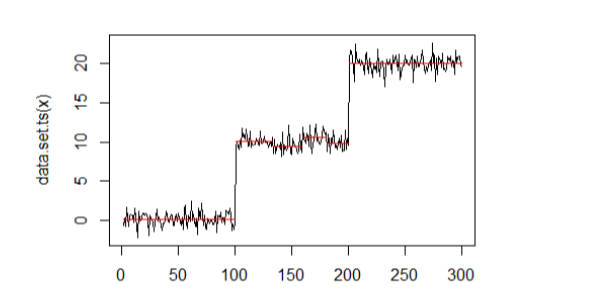
\includegraphics[width=1.0\textwidth]{media/puntos-cambios-segmenteos.png}
    \caption{Puntos de cambio detectados y división de la señal segmentos  \protect\cite{contreras2024cusum} }
    \label{fig:figPuntosCambiosSegmentos}
\end{figure}


La Media Móvil con Ponderación Exponencial (Exponentially Weighted Moving Average, EWMA) \cite{fan1996ewma} se utiliza en la detección de anomalías al suavizar datos y resaltar cambios significativos. La EWMA da más peso a las observaciones recientes, permite identificar desviaciones de la norma, facilitando la detección de patrones inusuales en series temporales. Esta técnica es aplicada en trading de divisas. 


\subsection{Métodos basados en aprendizaje de máquina}


Los sistemas industriales suelen ser complejos puesto que integran muchos componentes, y esto hace que la detección de anomalías sea una tarea bastante compleja porque técnicas univariadas para detección de anomalías no suelen ser suficientes. Muchas de las técnicas tradicionales de detección de anomalías, como las anteriormente mencionadas, fallan cuando los datos alcanzan una alta volumetría y también cuando se generan a muy alta velocidad y son multidimensionales \cite{thudumu2020survey}.


Para afrontar el problema de múltiples variables y sistemas más complejos, se implementa como alternativa los algoritmos de aprendizaje de máquina. Las ventajas de los algoritmos de aprendizaje de máquina sobre las estrategias basadas en reglas y estadísticas son múltiples. En primer lugar, mientras que los modelos de aprendizaje de máquina construyen las reglas que describen los patrones de los datos, en el modelamiento estadístico hay que formalizar las relaciones entre las variables a través de ecuaciones matemáticas, \cite{ij2018statvsml}. 


Otra ventaja de los algoritmos de aprendizaje de máquina sobre el modelado estadístico tradicional es que la capacidad de los modelos para aprender los patrones a partir de los datos proporcionados sin la necesidad de asumir una distribución específica de los datos. En el modelado estadístico normalmente se asume que los datos siguen alguna distribución, y es a partir de allí que se construyen las ecuaciones y reglas con que se modelan los datos. 


Existe una gran variedad de modelos de aprendizaje de máquina, una gran diversidad de estos modelos han sido implementados en el problema de detección de anomalías. Se puede encontrar en la literatura el uso de modelos de aprendizaje supervisado para la detección de anomalías. 


En el trabajo de \cite{baradaran2025predictivemaintenanceelectricmotors}, se  evaluaron varios modelos como Naive Bayes, SVM, Random Forest, k-NN, métodos de boosting, entre otros, para poder detectar alguno de los tres estados posibles de un motor: Saludable (Healthy), averiado (Broken), y necesita mantenimiento (Needs Preventive Maintenance). De este estrato se concluye que tiene sentido la aplicación de un modelo de clasificación de aprendizaje de máquina en ese caso de uso. Sin embargo, es importante la elección del modelo, puesto que se observan diferencias en las precisiones de los clasificadores.   


\subsubsection{Naive Bayes}

Naive Bayes es un algoritmo de aprendizaje automático que se basa en fundamentos estadísticos, principalmente en el teorema de Bayes el cual permite actualizar la probabilidad de una hipótesis a partir de nueva evidencia. Este teorema relaciona probabilidades de dos eventos A y B a través de la dependencia condicional, asumiendo independencia condicional, es decir, que los valores de una característica son independientes de la presencia o propiedades de las demás características. Según \cite{han2012datamining}, la Equación~\ref{eq:eq1NaiveBayes} describe al teorema de Bayes.


\begin{equation}\label{eq:eq1NaiveBayes}
P(A \mid B) = \frac{P(B \mid A) P(A)}{P(B)}
\end{equation}


Donde $P(A \mid B)$ es la Probabilidad posterior de que ocurra el evento $A$, dado que ya ocurrió el evento $B$; $P(B \mid A)$ es la Probabilidad condicional de que ocurra B si sabemos que el evento $A$ ya ocurrió; $P(A)$ es Probabilidad a priori de que ocurra $A$, sin considerar ninguna información adicional y $P(B)$ es Probabilidad total de que ocurra $B$, considerando todos los casos posibles.


Los clasificadores basados en el algoritmo Naive Bayes utilizan las probabilidades a priori para estimar la probabilidad de ocurrencia del evento objetivo. Aplican de manera secuencial la fórmula del Teorema de Bayes, asumiendo independencia condicional entre las características con el fin de simplificar los cálculos del modelo. Como resultado del proceso anterior, se obtiene la Equación~\ref{eq:eq1NaiveBayesProd} matemática para calcular la probabilidad estimada de que el evento objetivo ocurra. \cite{salman2024rf}. 


\begin{equation}\label{eq:eq1NaiveBayesProd}
P(C|x_1, x_2, ..., x_n) = P(C) \prod_{i = 0}^{n} P(x_i \mid C)
\end{equation}


A pesar de su simplicidad, el modelo de clasificación basado en Naive Bayes ofrece un rendimiento sorprendentemente eficaz en tareas de clasificación, y en muchos casos supera en precisión a métodos más complejos, especialmente cuando se trabaja con grandes volúmenes de datos y características independientes. Su eficiencia computacional lo convierte en una opción ideal para aplicaciones en tiempo real. Además, requiere una menor cantidad de datos para entrenamiento en comparación con otros algoritmos.


Otras investigaciones han encontrado qué el modelo de clasificación Naive-Bayes da buenos resultados de precisión. \cite{chen2016xgboost} entrenó dos modelos de clasificación para dos datasets diferentes, con Naive-Bayes. Los resultados fueron qué los modelos logran una precisión aproximada del 99.9\% y 99.65\%, respectivamente. Por otro lado, en múltiples trabajos, se encuentra qué el algoritmo qué mejor desempeño tiene a la hora de detectar anomalías es el random forest. Como por ejemplo el trabajo de \cite{sharma2022predictive} y \cite{yu2025tkeo}.


\subsubsection{Máquinas de soporte vectorial}

Las Máquinas de Vectores Soporte, SVM en por sus siglas en inglés: Support Vector Machine, tienen su principio en la aplicación de trabajos que requieren teoría de aprendizaje estadístico, son usadas para resolver tareas de clasificación y regresión. Según \cite{amat2017maquinas}, el principio fundamental en una SVM es encontrar un hiperplano óptimo encargado de la clasificación de los datos, el cual maximiza el margen entre las clases, es decir, la distancia entre los puntos de datos más cercanos de cada clase (conocidos como vectores soporte) y el hiperplano. En la Figura~\ref{figSVM} se observa cómo una Máquina de Vectores de Soporte clasifica datos en un hiperplano. 


\begin{figure}[h]
    \centering
    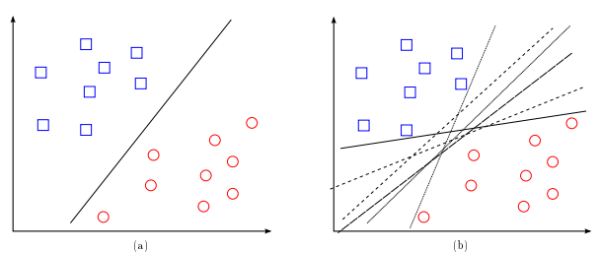
\includegraphics[width=1.0\textwidth]{media/svm-dm.png}
    \caption{Clasificación de datos en un espacio bidimensional. En (a) se observan los datos separados a través de un hiperplano óptimo, mientras que en (b) se muestra los posibles hiperplanos que se pueden aplicar para la separación de los datos.  \protect\cite{suarez2014svm} }
    \label{fig:figSVM}
\end{figure}


Mientras que la mayoría de métodos de aprendizaje se centran en minimizar los errores empíricos, las SVMs radican la minimización del riesgo estructural, es decir, se busca minimizar los errores empíricos, pero al mismo tiempo, maximizar la capacidad del modelo para generalizar. Este enfoque no solo mejora la capacidad de generalización del modelo ante nuevos datos y lo hacen robusto frente al sobreajuste. Otra ventaja que tienen los modelos SVM es el uso de funciones núcleo (kernel functions) que transforman el espacio permitiendo manejar problemas no linealmente separables. 


\begin{figure}[h]
    \centering
    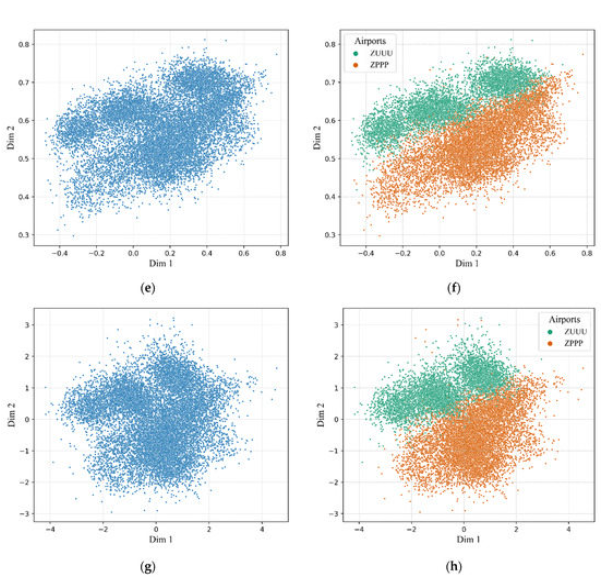
\includegraphics[width=1.0\textwidth]{media/svm-kun.png}
    \caption{Detección de anomalías en datos de vuelo utilizando One-Class SVM.  \protect\cite{qin2022flight} }
    \label{fig:figSVMflight}
\end{figure}


Originalmente este sistema fue creado para problemas de clasificación binaria, pero puede ser aplicado en problemas de clasificación multiclase, y también en problemas de detección de anomalías. En la Figura~\ref{fig:figSVMflight}, propuesta por \cite{qin2022flight}, se presenta un estudio para identificar anomalías en datos reales de vuelo, usando como base el principio One-Class SVM. Se construyó un sistema para detectar eventos anómalos en tiempo real, en la aplicación de este estudio se logró que es un método muy viable para este tipo de escenarios obteniendo una alta capacidad de detección de anomalías y mantuvo una baja tasa de falsas alarmas lo cual es crítico para monitoreo de aeronaves.


\subsubsection{k-NN}


K-Nearest-Neighbours (kNN) es quizás uno de los métodos más populares y sencillos para implementación de algoritmos de extracción y análisis de datos en una variedad de temas de investigación en informática. Los algoritmos KNN se han empleado de manera extensa en el ámbito de la investigación y se les reconoce como uno de los diez algoritmos más destacados en minería de datos \cite{witten2005data}. En este tiempo del Big Data, las metodologías KNN ofrecen una forma especialmente eficaz para reconocer patrones valiosos y crear algoritmos de razonamiento fundamentados en casos para la inteligencia artificial (IA). \cite{wu2008top}


El estudio de la selección de vecinos más cercanos ha sido ampliamente investigada, observada y analizada con el fin de determinar la mediana de proximidad, se puede decir que lo que se desea obtener con todo esto es centralizar la construcción de funciones de distancia para medir la proximidad. Es esencial contar con una función a distancia que permita elegir los puntos de vecinos más cercanos, la cual pueda operar de manera efectiva con la gran parte de las muestras de entrenamiento. \cite{zhang2022influence}

\begin{figure}[h]
    \centering
    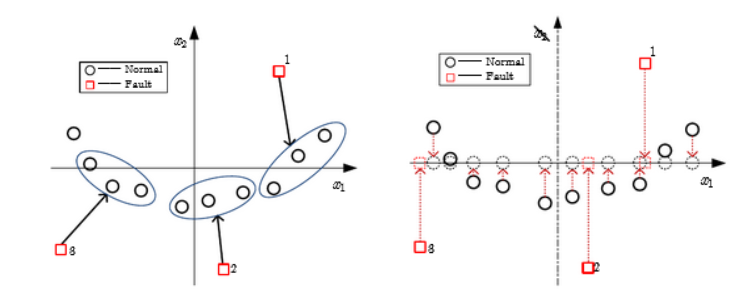
\includegraphics[width=1.0\textwidth]{media/knn-zhou.png}
    \caption{Detección de fallos usando FD‑kNN y PC‑kNN.  \protect\cite{zhou2015faultdetection} }
    \label{fig:figKnnZhou}
\end{figure}


En el campo de la detección de fallos, se han aplicado métodos basados en KNN : FD (Feature-Dependent) y PC (Prototype Constrained), cada uno sirvió para el estudio del comportamiento en situaciones controladas, logrando identificar altas tasas de detección de fallos y bajas tasas de falsas alarmas, proveyendo una solución simple y efectiva para detección de fallos en sistemas complejos, ofreciendo así resultados sólidos en aplicaciones industriales reales, validando su aplicabilidad práctica.\cite{zhou2015faultdetection}.


\subsubsection{Random Forest}


Los modelos basados en Random Forest son una de las herramientas más populares a la hora de construir modelos de predicción para clasificación, regresión y minería de datos \cite{rushall2013rf}. Consisten en un conjunto de árboles de decisiones entrenados con diferentes subconjuntos de datos aplicando estrategias como bagging y boosting. Los árboles de decisión dividen el hiperespacio en segmentos según los datos de prueba. Random Forest utiliza un conjunto de árboles de decisión para mejorar la capacidad de generalización.  


Según, \cite{salman2024rf}, una de las principales ventajas de los modelos basados en Random Forest es su versatilidad porque puede ser aplicado en regresión y clasificación,  además, tiene una buena tolerancia ante valores atípicos y el ruido, gracias a ésto han sido uno de los métodos de investigación más populares en el área de minería de datos. Adicionalmente, durante el entrenamiento de los árboles de decisión, las características más relevantes son ubicadas en la raíz del árbol de decisión, esto facilita la interpretación y búsqueda de patrones en los datos. 


Los modelos basados en algoritmos Random Forest, según \cite{canovas2017random}, tienen como una de sus principales ventajas que son simples de entrenar y al mismo tiempo pueden alcanzar un rendimiento similar al de otras técnicas más complejas, y también, son robustos ante un gran porcentaje de datos nulos. Por esta razón, esta técnica es ampliamente utilizada en la detección de fraudes bancarios y otros tipos de anomalías en los datos. 


\cite{yu2025tkeo} compararon el rendimiento de los modelos de clasificación SVM  y Random Forest, aplicando el operador TKEO sobre el dataset CWRU como técnica de preprocesamiento para predecir alguno de 17 categorías relacionadas con la salud del motor. Ambos modelos tuvieron buenos resultados y demostraron qué bajo ciertas condiciones de cargas es viable utilizar el TKEO debido a su eficiencia con dataset grandes.


\cite{sharma2022predictive} realiza la evaluación de cinco modelos de clasificación usando datasets diferentes para predecir el momento para mantenimiento. El objetivo es determinar cuál de los modelos funciona mejor. En este estudio curiosamente se vuelve a resaltar a Random Forest como el modelo con la mayor precisión.


\subsubsection{XGBoost}

El algoritmo XG Boost (Extreme Gradient Boosting) es una técnica de aprendizaje supervisado que se basa en árboles de decisión \cite{chen2016xgboost}.  Es una poderosa herramienta de aprendizaje automático que fusiona eficacia, adaptabilidad y excelente desempeño para solucionar problemas complicados de clasificación y regresión. 

\begin{figure}[h]
    \centering
    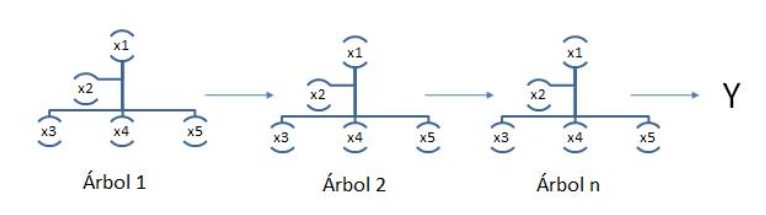
\includegraphics[width=1.0\textwidth]{media/xgboost-salman.png}
    \caption{Visualización del algoritmo XGBoost. Ensamble de árboles de decisión.  \protect\cite{salman2024rf} }
    \label{fig:figXGBoostSalman}
\end{figure}


Se basa principalmente en la implementación del algoritmo de boosting de árboles de decisión. XGBoost consiste en un ensamblaje secuencial de árboles de decisión. Los árboles se agregan secuencialmente a fin de aprender del resultado de los árboles previos y corregir el error producido por los mismos, hasta que ya no se pueda corregir más dicho error \cite{salman2024rf}.  En XGBoost, a esta técnica donde cada árbol recién construido busca rectificar los fallos realizados por los árboles previos con el objetivo de generar un modelo más robusto y exacto se le denomina “gradiente descendiente”. \cite{espinoza2020rf_xgboost}.

\subsubsection{CatBoost}

CatBoost es otro algoritmo de Machine Learning basado en árboles de decisión, su principal ventaja es su eficiente capacidad de predicción para características de tipo categórico  \cite{ibrahim2020catboost}. A diferencia de otros modelos basados en Boosting, esta técnica no requiere aplicar técnicas de hot-encoding manualmente, puesto que es capaz de manejar las variables categóricas de forma nativa. CatBoost implementa gradient boosting, el cual hace uso de árboles de decisión binarios como base para sus predictores \cite{prokhorenkova2018catboost}.


CatBoost se ha implementado en la detección de robo de electricidad. Fue seleccionado este modelo por su eficiencia para manejar un gran porcentaje de características de datos de tipo categórico durante el entrenamiento del modelo como en su predicción, \cite{hussain2021catboost}. Asimismo, otra ventaja de este algoritmo es su interpretabilidad, en contraste con otras soluciones basadas en boosting. 


\subsubsection{LightGBM}


Este es uno de los algoritmos más populares de aprendizaje automático, es ampliamente implementado en soluciones que manejen grandes volúmenes de datos y de gran dimensionalidad. LightGBM usa estrategias claves, GOSS (Gradient-based One-Side Sampling) que consiste en usar las observaciones con mas gradientes grandes ya que son las instancias donde el modelo pierde exactitud en la predicción, y por otro lado EFB (Exclusive Feature Bundling) que agrupa las variables que usualmente toman valores nulos o iguales a cero. Estas variables son empaquetadas lo que reduce considerablemente la cantidad de variables a considerar.


Se estima que LightGBM logra entrenar mucho más rápido (hasta 20 veces), que otros modelos basados en árboles de decisión, lo que permite el procesamiento de grandes volúmenes de datos y un buen rendimiento en contextos donde la velocidad es crítica, como en sistemas en tiempo real, \cite{ke2017lightgbm}. En IoT, por ejemplo, se ha implementado LightGBM para la detección de anomalías en sistemas de enfriamiento. \cite{yanabe2020lightgbm}, y también se ha implementado este método para la detección de anomalías en el tráfico de una red. \cite{islam2020lightgbm}. 


\cite{delasmorenas2025bearing} probaron tres modelos de clasificación (XGBoost, CatBoost y LightGBM). Los 3 demostraron buenos resultados en precisión (98\% aprox.). Este estudio termina con la conclusión que para ese caso de uso el algoritmo de LightGBM obtiene los mejores resultados, y que se debe considerar como opción en casos de Edge Computing.


\subsection{Métodos basados en aprendizaje no supervisado}

En los anteriores trabajos se encuentra qué los dataset con los qué trabajaron eran dataset previamente etiquetados. Sin embargo esto puede ser una limitación en aplicaciones industriales o de negocio en las que el trabajo de etiquetado no se ha hecho.


Existen casos de detección de anomalías donde se busca que el modelo segmenta un conjunto de datos no etiquetados previamente de manera que sea éste el que defina qué es una anomalía y que no. Esta técnica de segmentación en la que los conjuntos de datos no han sido previamente etiquetados se denomina aprendizaje no supervisado. Aplicando este enfoque,  \cite{Cao_2025} escribe un artículo hablando de distintas técnicas para la detección de anomalías a través de mecanismos de aislamiento. Se mencionan varias técnicas, pero de las más destacadas se encuentra la Insolation Forest.


\subsubsection{Isolation Forest}




\chapter{Identificación de Requisitos}


\chapter{Objetivos}

Dada la creciente necesidad de identificar comportamientos atípicos en la industria, 
se plantean una serie de objetivos claros que permiten abordar el problema desde una 
perspectiva integral. 
Estos objetivos guían el diseño, implementación y evaluación de modelos capaces de 
detectar desviaciones anomalías de manera eficiente y precisa.


\section{Objetivo General}

\textbf{Desarrollar} una solución basada en algoritmos de aprendizaje automático 
capaz de detectar anomalías en datos provenientes de entornos industriales, garantizando
un desempeño medible a través de métricas estándares.
La solución deberá alcanzar métricas de rendimiento superiores a 0.85 en métricas como
exactitud y F1, demostrando alta eficacia en la identificación de anomalías.

\section{Objetivos Específicos}

\begin{itemize}

\item Desarrollar la arquitectura de una solución para la detección de anomalías, donde 
se definan claramente los distintos componentes que la integran, sus funciones y el 
flujo de trabajo que sigue la solución, con el fin de  garantizar una implementación 
clara y coherente.


\item Analizar conjuntos de datos industriales, con el fin de garantizar que cumpla 
con los requerimientos necesarios para la implementación de algoritmos de aprendizaje 
automático y realizar los ajustes y transformaciones a los datos en caso de ser necesario. 


\item Seleccionar los modelos y algoritmos de aprendizaje automático que se integrarán
en la solución, e implementar los ajustes necesarios en sus parámetros y configuración
con el fin de optimizar su rendimiento en términos de precisión, sensibilidad y otras
métricas relevantes.


\item Evaluar el desempeño de los modelos seleccionados, utilizando un conjunto de 
condiciones experimentales homogéneas que garanticen una evaluación objetiva, 
identificando fortalezas, limitaciones y oportunidades de mejora.


\item Implementar el análisis del conjunto de datos, la selección, entrenamiento y 
evaluación de modelos, la ejecución de pruebas controladas y la disponibilización de la 
solución final, utilizando herramientas de desarrollo especializadas. 

\end{itemize}


\chapter{Metodología de trabajo}


El presente trabajo se enmarca en un enfoque cuantitativo y de tipo aplicado, ya que se 
busca diseñar, implementar y evaluar una solución basada en algoritmos de aprendizaje 
automático para la detección de anomalías en datos industriales. La investigación se 
centra en el procesamiento y análisis de datos numéricos provenientes de sistemas reales,
con el objetivo de generar métricas que sean medibles y replicables, ejemplos de estas 
métricas son precisión, sensibilidad, especificidad, F1-score y área bajo la curva ROC.
El estudio es descriptivo, en la medida en que se analizan características estadísticas 
de los datos, se aplican técnicas de preprocesamiento, y es experimental, porque se 
construyen modelos que son evaluados bajo métricas estándar de desempeño. 


\section{Metodología CRISP-DM}

Con el fin de alcanzar los objetivos propuestos del presente proyecto, se ha decidido 
basarse en los pasos de la metodología  CRISP-DM, llamada así por sus siglas en inglés 
CRoss-Industry Standard Process for Data Mining. La ventaja de aplicar las fases de esta
metodología es su enfoque a proyectos de ciencia y minería de datos e inteligencia 
artificial, y que además ofrece una guía para ajustar los procedimientos técnicos del 
proyecto a los objetivos propuestos, lo que facilita la selección de actividades y 
la ejecución del proyecto. La Figura~\ref{fig:figCrispdm} muestra cada una de las fases de la metodología 
CRISP-D.


\begin{figure}[h]
    \centering
    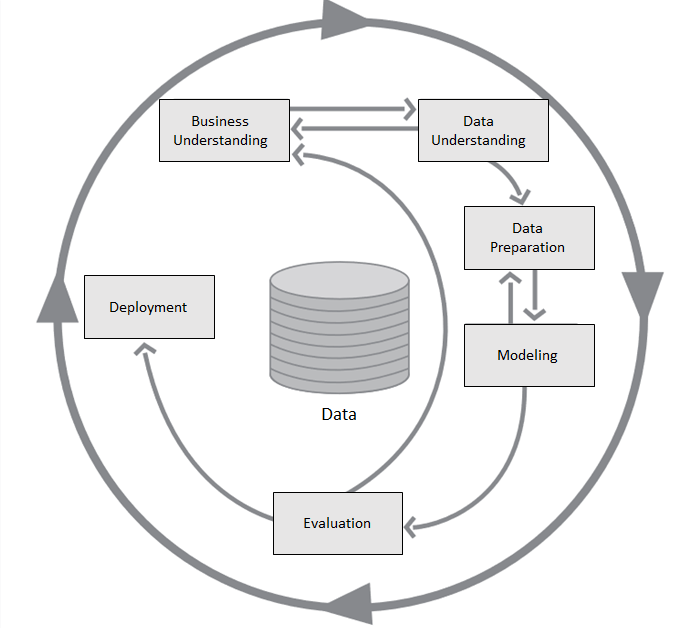
\includegraphics[width=0.6\textwidth]{media/crisp-dm.png}
    \caption{Fases de la metodología {CRISP-DM}.  \protect\cite{chapman2000crisp} }
    \label{fig:figCrispdm}
\end{figure}



\subsection{Entendimiento del tema}

Aquí es donde se hace un análisis del contexto, se desarrollan los objetivos generales 
y específicos del proyecto. Esos objetivos deben girar en torno al desarrollo de una 
solución capaz de identificar comportamientos atípicos de variables industriales con un 
desempeño superior a los de métodos actuales. Acá se definen los criterios de éxito del
sistema, las métricas que se van a utilizar para evaluar los modelos, las reglas a la 
hora de realizar la comparación, y las condiciones que se espera que el modelo cumpla 
para ser implementado en ambientes industriales reales. 


\subsection{Entendimiento de los datos}


Para la etapa de entendimiento de datos se realiza una selección de un conjunto de datos
de variables industriales, los cuales pueden incluir mediciones de sensores, logs de 
máquinas, registros y tendencia de producción, entre otros. A estos datos de entrada se 
les realiza un análisis exploratorio con el propósito de identificar las variables 
relevantes, correlaciones, valores atípicos, duplicados y faltantes y calcular 
estadísticos descriptivos de las variables y su distribución.


La fase de entendimiento de los datos permite conectar los objetivos del proyecto con 
los conjuntos de datos disponibles. Aquí se define operativamente qué se considera una 
anomalía, teniendo en cuenta el contexto de los procesos industriales y las posibles 
causas de desviaciones. Es importante identificar en el conjunto de datos si se cuenta 
con una etiqueta que identifique si los datos corresponden a una anomalía o no, esto es 
importante para la fase de modelado porque esto determina si se cumplen las condiciones 
para seleccionar un algoritmo supervisado o no supervisado. 

\subsection{Preparación de los datos}


Con base en el análisis exploratorio de los datos, se seleccionan los procedimientos 
que harán parte de la fase de preprocesamiento de los datos, y también aquellos 
algoritmos que realicen transformaciones sobre los datos. Durante esta fase se eligen 
las estrategias para lidiar con datos faltantes, y las técnicas de reducción de ruido. 
En esta fase también se estudia la posibilidad de aplicar técnicas como feature engineer 
y análisis de componentes principales (PCA),  con el fin facilitar la inferencia de los 
modelos de las fases siguientes.


\subsection{Modelado}


Tal como se plantea en el segundo objetivo específico, en esta fase se implementa un 
modelo de machine learning basándose en los datos ya procesados. Se hace una selección 
rigurosa de los algoritmos a utilizar. Una vez seleccionados, se implementan y se 
comparan soluciones del estado del arte y finalmente, se hacen los respectivos ajustes 
para optimizar su rendimiento.
El conjunto de todos estos pasos hace posible la construcción de un modelo robusto que 
cumpla con los requerimientos del proyecto. 


\subsection{Evaluación}

Los modelos entrenados se evalúan mediante un conjunto homogéneo de datos y condiciones 
experimentales, siguiendo el tercer objetivo específico. Se hace una interpretación de 
los resultados de la evaluación, y se identifican con éstos, las ventajas y desventajas 
que presentan unos modelos frente a otros. 
Se hace un énfasis en el modelo propuesto en los resultados del modelo propuesto. 
Los resultados determinan en qué grado el modelo cumple con los requerimientos propuestos. 

\subsection{Despliegue}

Se propone una estrategia de despliegue donde el modelo esté disponible y pueda ser 
integrado fácilmente con otras herramientas que hacen parte del contexto industrial. 
Se abordan temas de escalabilidad, mantenimiento y actualización continua del modelo. 
Este paso garantiza el cumplimiento del objetivo general. 



\chapter{Desarrollo del trabajo}



\chapter{Discusión y análisis de resultados}

Los modelos entrenados tienen muy buenas métricas de rendimiento. 
Los resultados obtenidos en la evaluación de los diferentes modelos de aprendizaje 
automático aplicados a la detección de anomalías muestran un desempeño sobresaliente 
en todas las métricas. 
Al revisar los valores de la Tabla 4, se observa que variables como la exactitud, 
la precisión, la sensibilidad, el F1-score y el área bajo la curva ROC alcanzan 
valores muy altos, superiores en la mayoría de los casos al 0.99. Esto refleja que los 
errores cometidos por los modelos son mínimos, los modelos logran una detección 
confiable de las anomalías y, por tanto, se cumplen los objetivos planteados en 
este proyecto.


El proceso de generar características a partir de los segmentos de serie de tiempo, 
en lugar de utilizar directamente los datos crudos, contribuyó de manera significativa 
a alcanzar estas métricas tan altas. Al aplicar las transformaciones a los datos y 
obtener indicadores estadísticos y espectrales, se logró capturar información relevante 
que permite a los modelos diferenciar con claridad entre estados normales y anómalos, 
mejorando sustancialmente la capacidad predictiva. Entre los parámetros que más 
contribuyeron a la inferencia de la clasificación están la media, la desviación estándar, 
el RMS, la frecuencia fundamental y la distorsión armónica total.


Con respecto al desempeño específico de los modelos, aquellos basados en técnicas de 
gradient boosting, particularmente XGBoost y LightGBM, alcanzaron las métricas más altas, 
mostrando un equilibrio casi perfecto entre precisión y sensibilidad y obtuvieron las 
métricas más altas entre todos los modelos seleccionados. Sin embargo, incluso modelos 
más simples, como la regresión logística, Naive Bayes o KNN, lograron resultados 
sobresalientes, con métricas por encima del 95\%, lo que indica que los datos están muy 
bien representados y que diferentes enfoques de modelado pueden ser útiles en este 
contexto.


Estos resultados demuestran además de ajustarse a los datos, los modelos permiten 
realizar interpretaciones valiosas sobre los factores más influyentes en la detección 
de anomalías. 
Al realizar un análisis detallado de los modelos de regresión logística, árbol de 
decisión y Naive Bayes, se identifican las variables para los modelos a la hora de 
realizar las predicciones. Esas variables fueron la desviación estándar, el valor 
máximo (pico), el RMS, la frecuencia fundamental y la distorsión armónica total THD. 
Esto le da a algunos modelos una doble ventaja: por un lado, una alta capacidad 
predictiva, y por otro, un mayor entendimiento del comportamiento del sistema.


Finalmente, se hace énfasis en la escasa diferencia entre las métricas de los distintos
modelos, resulta difícil declarar un ganador absoluto únicamente con base en su 
rendimiento. 
Para seleccionar el modelo más adecuado para una implementación práctica, deben 
considerarse otros factores además del rendimiento, como la necesidad de ejecutar el 
sistema en tiempo real, la disponibilidad de recursos computacionales y la 
interpretabilidad del modelo. 


En este sentido,  si se busca un modelo con alta interpretabilidad, se aplica el 
principio de parsimonia para seleccionar modelos como Regresión Logística, Naive Bayes,
o Árboles de Decisión, ya que con éstos es  más fácil de explicar el aporte de cada 
variable al  resultado final.  
Si se requiere rapidez y bajo consumo de cómputo, se aplica el mismo principio, y 
nuevamente modelos como regresión logística o los árboles de decisión suelen ser más 
adecuados porque combinan unas muy buenas métricas con un bajo requerimiento de cómputo.
En escenarios donde se requiera una máxima precisión, modelos más complejos como 
XGBoost o LightGBM se perfilan como la mejor opción.



\chapter{Conclusiones y Trabajo Futuro}

En el presente  trabajo se alcanzaron métricas superiores al 90\% en todos los modelos
evaluados, superando el resultado esperado, lo cual refleja la solidez del enfoque 
planteado para la detección de anomalías en entornos industriales. La etapa de 
preprocesamiento de los datos fue un paso clave: la caracterización de las series de 
tiempo, junto con un adecuado balanceo del dataset y la búsqueda de hiperparámetros, 
permitió que los modelos pudieran generalizar mejor y mostraran robustez frente al 
sobreajuste. Estos resultados confirman la efectividad del pipeline desarrollado para 
transformar datos crudos en características discriminativas útiles para los modelos 
de predicción.


Debido al alto rendimiento alcanzado, todos los modelos evaluados podrían aplicarse en 
una solución in-situ. No obstante, los que obtuvieron las mejores métricas fueron 
XGBoost y LightGBM, confirmando su eficacia como algoritmos de referencia en problemas
de clasificación complejos, y un buen referente para la detección de anomalías. Sin 
embargo, si la implementación requiere simplicidad, interpretabilidad y bajo costo 
computacional, los modelos clásicos como la regresión logística, los árboles de decisión
o Naive Bayes resultan altamente recomendables, ya que ofrecen un equilibrio entre 
eficiencia, precisión e interpretabilidad.


Finalmente, gracias al uso de modelos con mayor interpretabilidad, se identificó que 
variables como los valores pico (maximum), la desviación estándar ($std$), el valor RMS ($rms$),
la frecuencia fundamental ($f0$) y la distorsión armónica total ($tdh$) son las que más 
aportan a la clasificación de una observación como anomalía. Este hallazgo  además de 
validar la calidad del modelo, proporciona información valiosa para la toma de 
decisiones en el ámbito industrial, al permitir inferir cuáles son los factores físicos
más determinantes en el diagnóstico temprano de fallos.


Como línea de trabajo futuro, una posibilidad interesante es la integración de los 
modelos desarrollados en un PLC (Controlador Lógico Programable) u otro dispositivo
de cómputo industrial. Esto permitiría que la detección de anomalías se ejecute de 
manera automática y en tiempo real dentro del propio entorno productivo. La adaptación
de los algoritmos a este tipo de hardware representa un reto, especialmente en lo 
relacionado con la optimización del uso de recursos computacionales, pero a la vez abre
la puerta a aplicaciones industriales de gran impacto.


Otra línea de investigación a considerar es el diseño de un algoritmo de clasificación
que no solo detecte anomalías, sino que también identifique el tipo específico de falla:
un clasificador multiclase.  Este enfoque aportaría un valor agregado, ya que permitiría
pasar de un sistema de simple diagnóstico (anómalo/no anómalo) a un sistema de prognosis
y clasificación de fallas, capaz de diferenciar entre problemas la gravedad del fallo y 
el lugar donde se presenta. Con ello, las soluciones podrían evolucionar hacia un 
mantenimiento predictivo más preciso y especializado.


En la Ecuación \eqref{eq:eq1secCTF}


\begin{equation}\label{eq:eq1secCTF}
M=\begin{pmatrix}
	m_{11}&m_{12}\\
	m_{21}&m_{22}
\end{pmatrix}
\end{equation}

En la siguiente Tabla \ref{tab:tab1secCTF}

\begin{table}[h]
\centering
\begin{tabular}{|c|c|}
	\hline
	1 & 2 \\
	\hline
	22 & 11 \\
	\hline
\end{tabular}
\caption{Tabla 1}
\label{tab:tab1secCTF}
\end{table}

En la siguiente Figura \ref{fig:fig1secCTF}

\begin{figure}[h]

\includegraphics[width= 0.8\textwidth]{logo_unir}
\caption{Logo Unir}
\label{fig:fig1secCTF}
\end{figure}

\cite{PIMENTEL2016744} \cite{da_S_Bessa_2023}

%\begin{thebibliography}{a}
%\bibitem{etiqueta} \textsc{Autores},
%\textit{nombre referencia.}
%Información addicional
%\end{thebibliography}
\bibliographystyle{apacite}
\bibliography{bibliografia}

\appendix
\chapter{Apendices}

\end{document}





















